%%%%%%%%%%%%%%%%%%%%%%%%%%%%%%%%%%%%%%%%%%%%%%%%%%%%%%%%%%%%%%%%%%%%%%%%%%%%%
%	e-Yantra, IIT-Bombay

%	Document Author: Chinmay Patil
%	Date: 11-July,2016
%	Last Edited by: Chinmay
%   Date Last updated: 11-06-2016 

%%%%%%%%%%%%%%%%%%%%%%%%%%%%%%%%%%%%%%%%%%%%%%%%%%%%%%%%%%%%%%%%%%%%%%%%%%%%%


\documentclass[11pt,a4paper]{article}
\usepackage{graphicx}
\usepackage{listings}
\usepackage{graphics}
\usepackage{wrapfig}
\usepackage[T1]{fontenc}
\usepackage[margin=1.2in]{geometry}
\usepackage{tcolorbox}
\usepackage{hyperref}
\usepackage{dingbat}
\usepackage{float}
\usepackage{tocloft}


\begin{document}
\begin{titlepage}
\title{Introduction to Wiced Sense}
\author{e-Yantra Team}
\date{\today}
\maketitle
\end{titlepage}
 \tableofcontents

\newpage
\section{What is Wiced Sense?}
\begin{figure}[h]
    \centering
	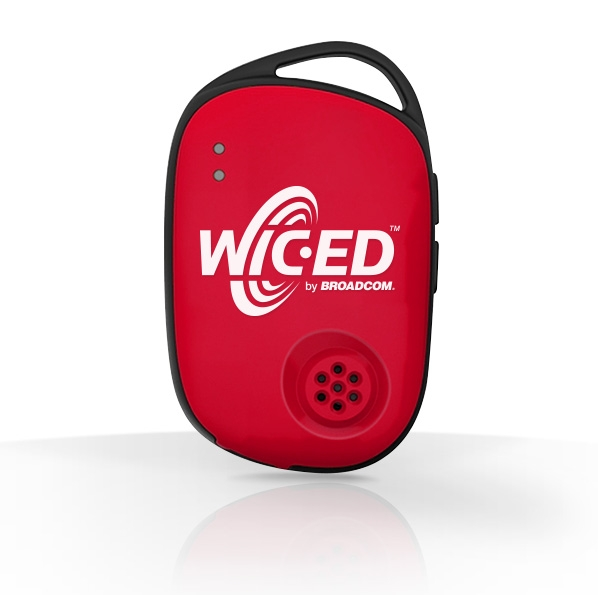
\includegraphics[scale=0.5]{WICED_SENSE.jpg}
	\caption{Wiced Sense Tag}
	\end{figure}


\begin{itemize}
\item WICED Sense is a BLE device manufactured by Broadcom* which can provide wireless connectivity to wide range of embedded applications.
\item The WICED Sense TAG is made up of the BCM20737S Bluetooth Low Energy SoC and five ST Microelectronics sensors: gyroscope, accelerometer, magnetometer , pressure, humidity and temperature. The BCM20737S connects directly to the sensors without the need for an external microprocessor.(* 5 July,2016 onwards Broadcoms IoT business is acquired by Cypress.)
\item ST Microelectronics Devices used in the WICED Smart Kit:
\begin{itemize}
\item Gyroscope (L3GD20)
\item Accelerometer (LIS3DSH)
\item Magnetometer (LSM303D)
\item Pressure sensor (LPS25H)
\item Humidity and Temperature sensor (HTS221)
\end{itemize}


\newpage
\section{Description about BCM20737}

\begin{figure}[h]
    \centering
	
\includegraphics[scale=0.5]{BCM20737.jpg}
		\caption{}
	\end{figure}



\item The BCM20737 is a an advanced Bluetooth low energy (aka Bluetooth Smart) 
SoC(System On Chip) that supports wireless charging, includes advanced security features and introduces new software support for NFC (Near Field Communiction) pairing. 
\item The BCM20737 is designed to support the entire spectrum of Bluetooth Smart use cases for the medical, home automation, accessory, sensor, Internet Of Things, and wearable market
segments. The BCM20737 radio has been designed to provide
low power, low cost, and robust communications for applications operating in the globally available
2.4 GHz unlicensed Industrial, Scientific, and Medical
(ISM) band.
\item The single-chip Bluetooth low energy SoC is a
monolithic component implemented in a standard
digital CMOS process and requires minimal external
components to make a fully compliant Bluetooth
device. The BCM20737 is available in a 32-pin,
5 mm x 5 mm 32-QFN package as well as WLBGA
SIP and die packages.

\item Microprocessor Unit
\begin{itemize}
\item The BCM20737 microprocessor unit (MPU) executes software from the link control (LC) layer up to the
application layer components. The microprocessor is based on an ARM Cortex M3, 32-bit RISC processor with embedded ICE-RT debug and JTAG interface units. The MPU has 320 KB of ROM for program storage and
boot-up, 60 KB of RAM for scratch-pad data, and patch RAM code. The SoC has a total storage of 380 KB,
including RAM and ROM.
\end{itemize}

\item Applications
\\ \\
The following profiles are supported in ROM :
\begin{itemize}
\item  Battery status
\item Blood pressure monitor
\item Find me
\item Heart rate monitor
\item Proximity
\item Thermometer
\item Weight scale
\item Time
\end{itemize}

\newpage
\item BCM20737 Architecture
\begin{figure}[h]
    \centering
	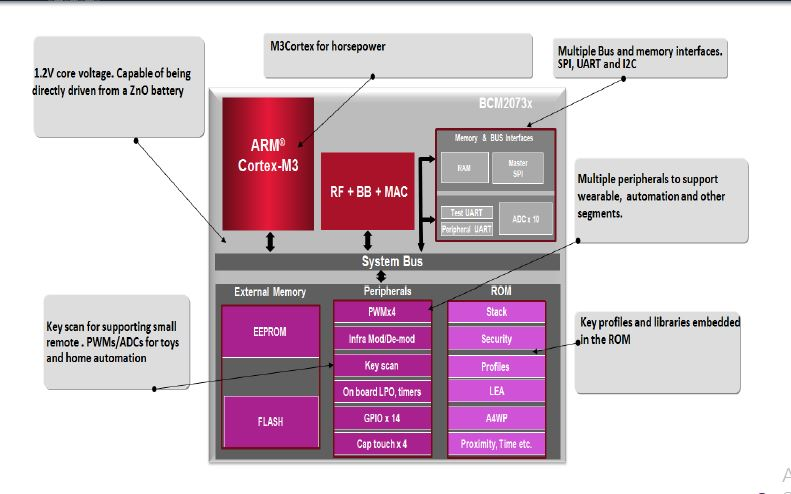
\includegraphics[scale=0.8]{architecture.JPG}
	\caption {BCM20737 Architecture}
	\end{figure}
	
	
	
	
\newpage
\section{Sensor 1 : Accelerometer(LIS3DSH)}


\begin{figure}[h]
    \centering
	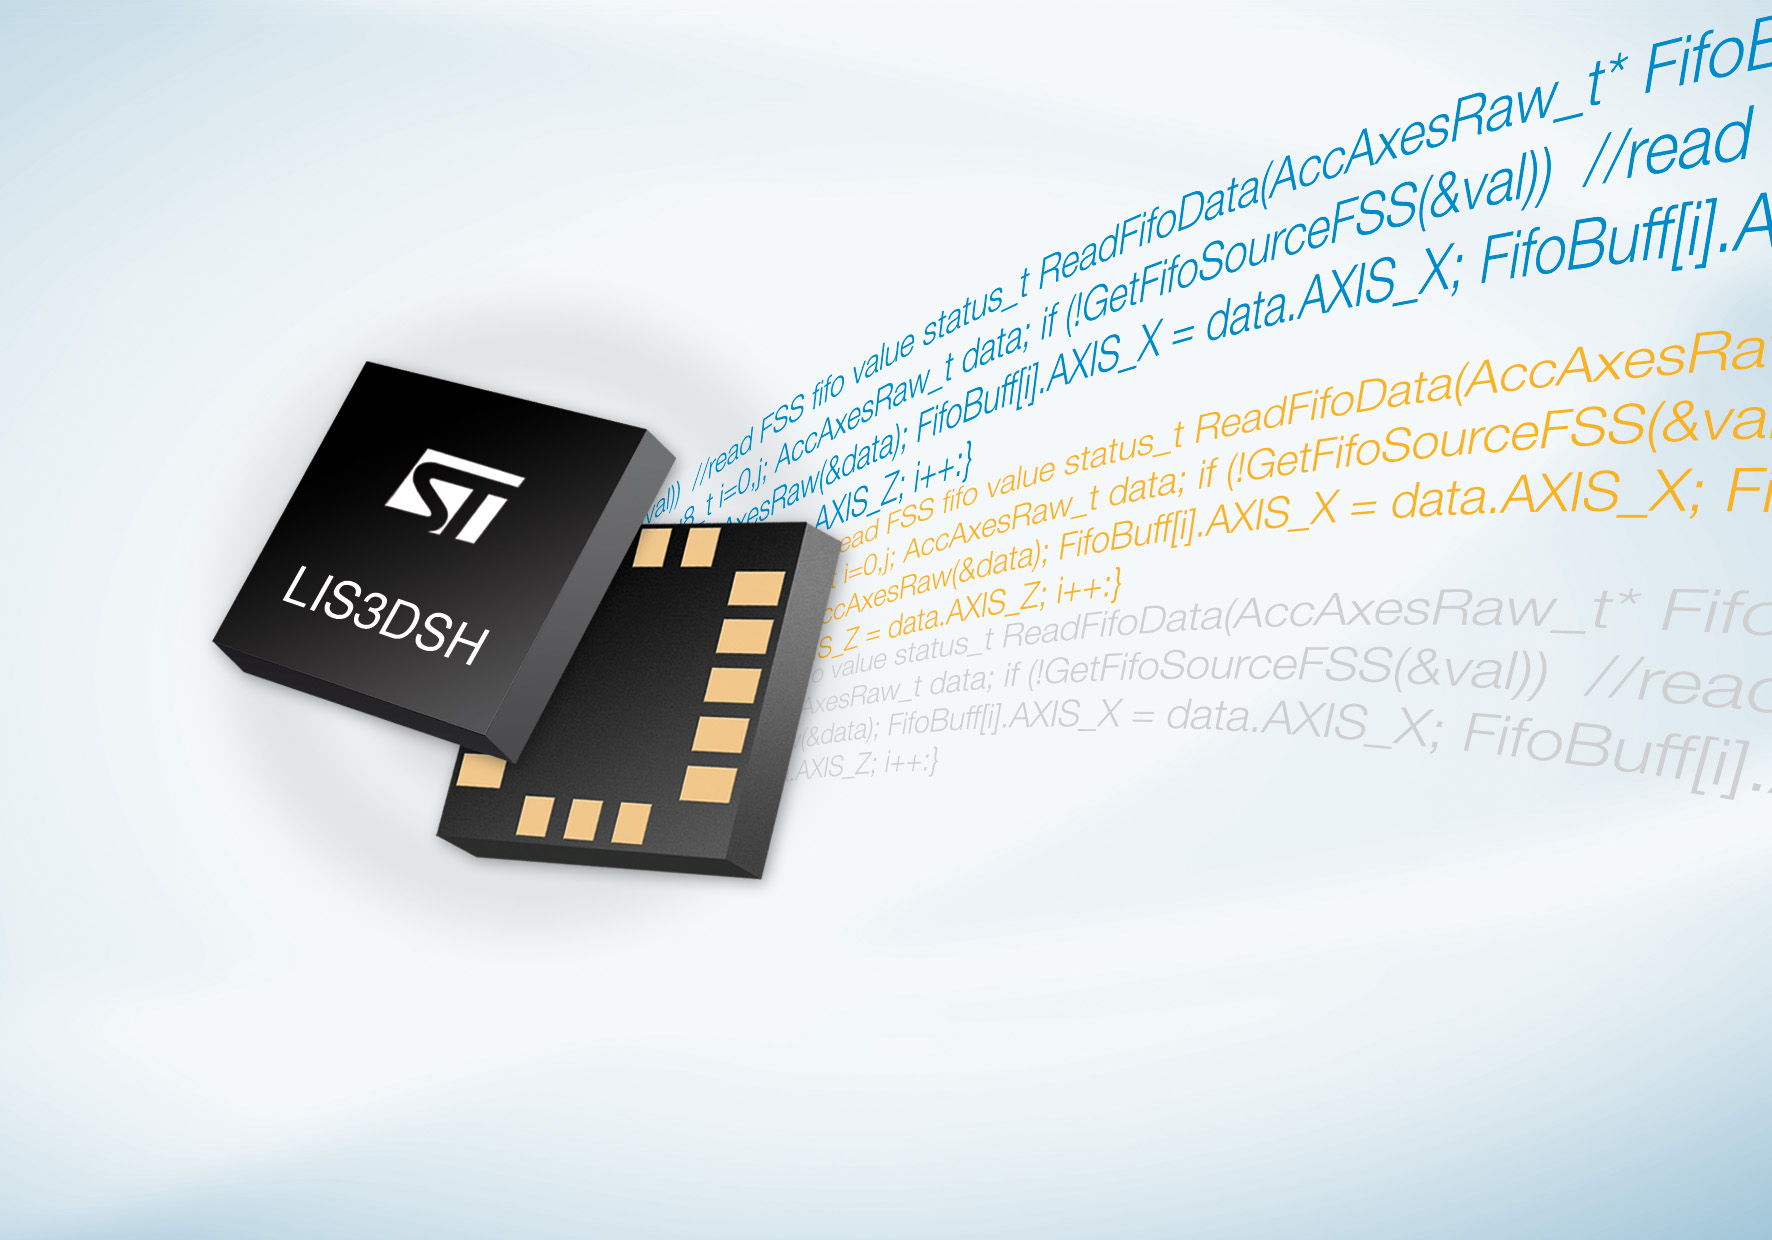
\includegraphics[scale=0.5]{LIS3DSH.jpg}
	\caption {STMicroelectronics LIS3DSH}
	\end{figure}
	
\item An accelerometer is a dynamic sensor capable of a vast range of sensing. Accelerometers measure acceleration in one, two, or three orthogonal axes.

\item The LIS3DSH is an ultra low-power high
performance three-axis linear accelerometer
belonging to the nano family with embedded
state machine that can be programmed to
implement autonomous applications.


\item The LIS3DSH has dynamically selectable full
scales of 2g/4g/6g/8g/16g ( 'g' represents gravitational force ) and it is capable
of measuring accelerations with output data rates
from 3.125 Hz to 1.6 kHz.


\item The self-test capability allows the user to check
the functioning of the sensor in the final
application.


\item The device can be configured to generate
interrupt signals activated by user defined motion
patterns.

\item The LIS3DSH has an integrated first in, first out
(FIFO) buffer allowing the user to store data for
host processor intervention reduction.

\item The LIS3DSH is available in a small thin plastic
land grid array package (LGA) and it is
guaranteed to operate over an extended
temperature range from -40 C to +85 C.

\item Its applications are :
\begin{itemize}
\item Motion controlled user interface
\item Gaming and virtual reality
\item Pedometer
\item Intelligent power saving for handheld devices
\item Display orientation
\item Click/double click recognition
\item Impact recognition and logging
\item Vibration monitoring and compensation

\end{itemize}

\newpage
\section{Sensor 2 : Gyroscope (L3GD20)}

\begin{figure}[h]
    \centering
	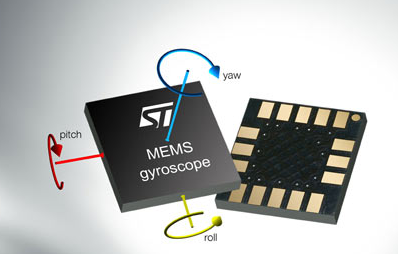
\includegraphics[scale=0.5]{gyroscope.png}
	\caption {STMicroelectronics L3GD20}
	\end{figure}

\item The L3GD20 is a low-power three-axis angular
rate sensor.

\item It includes a sensing element and an IC interface
capable of providing the measured angular rate to
the external world through a digital interface
(I2C/SPI).

\item The sensing element is manufactured using a
dedicated  micro-machining process developed by
STMicroelectronics to produce inertial sensors
and actuators on silicon wafers.

\item The IC interface is manufactured using a CMOS
process that allows a high level of integration to
design a dedicated circuit which is trimmed to
better match the sensing element characteristics.
The L3GD20 has a full scale of 250/500/2000
dps (degree per second) and is capable of measuring rates with a
user-selectable bandwidth.

\item The L3GD20 is available in a plastic land grid
array (LGA) package and can operate within a
temperature range of -40 degree Celsius to +85 degree Celsius.

\item Features 
\begin{itemize}
\item Three selectable full scales (250/500/2000
dps)
\item I2C/SPI digital output interface
\item 16 bit-rate value data output
\item 8-bit temperature data output
\item Two digital output lines (interrupt and data
ready)
\item Integrated low- and high-pass filters with user selectable
bandwidth
\item Wide supply voltage: 2.4 V to 3.6 V
\item Low voltage-compatible IOs (1.8 V)
\item Embedded power-down and sleep mode
\item Embedded temperature sensor
\item Embedded FIFO
\item High shock survivability

\end{itemize}

\item Applications
\begin{itemize}
\item Gaming and virtual reality input devices
\item Motion control with MMI (man-machine
interface)
\item GPS navigation systems
\item Appliances and robotics
\end{itemize}


\newpage
\section{Sensor 3 : Magnetometer (LSM303D)}


\begin{figure}[h]
    \centering
	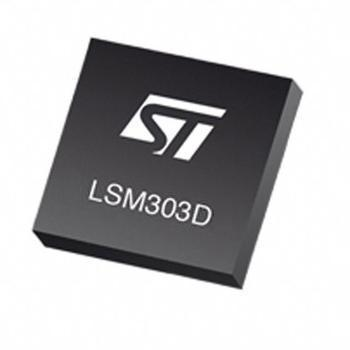
\includegraphics[scale=0.5]{LSM303D.png}
	\caption {STMicroelectronics LSM303D}
	\end{figure}
	
\item The LSM303D is a system-in-package featuring a
3D digital linear acceleration sensor and a 3D
digital magnetic sensor.

\item The LSM303D has linear acceleration full scales
of 2g / 4g / 6g / 8g / 16g and a magnetic
field full scale of 2 / 4 / 8 / 12 gauss.
\item The LSM303D includes an I2C serial bus
interface that supports standard and fast mode
(100 kHz and 400 kHz) and SPI serial standard
interface.

\item The system can be configured to generate an
interrupt signal for free-fall, motion detection and
magnetic field detection. Thresholds and timing of
interrupt generators are programmable by the end
user.

\item Magnetic and accelerometer blocks can be
enabled or put into power-down mode separately.
\item The LSM303D is available in a plastic land grid
array package (LGA) and is guaranteed to
operate over an extended temperature range
from -40 degree Celsius to +85 degree Celsius.

\item Applications
\begin{itemize}

\item Tilt-compensated compasses
\item Map rotation
\item Position detection
\item Motion-activated functions
\item Free-fall detection
\item Click/double-click recognition
\item Pedometers
\item Intelligent power saving for handheld devices
\item Display orientation
\item Gaming and virtual reality input devices
\item Impact recognition and logging
\item Vibration monitoring and compensation

\end{itemize}

\newpage
\section{Sensor 4 : Pressure Sensor (LPS25H)}
\begin{figure}[h]
    \centering
	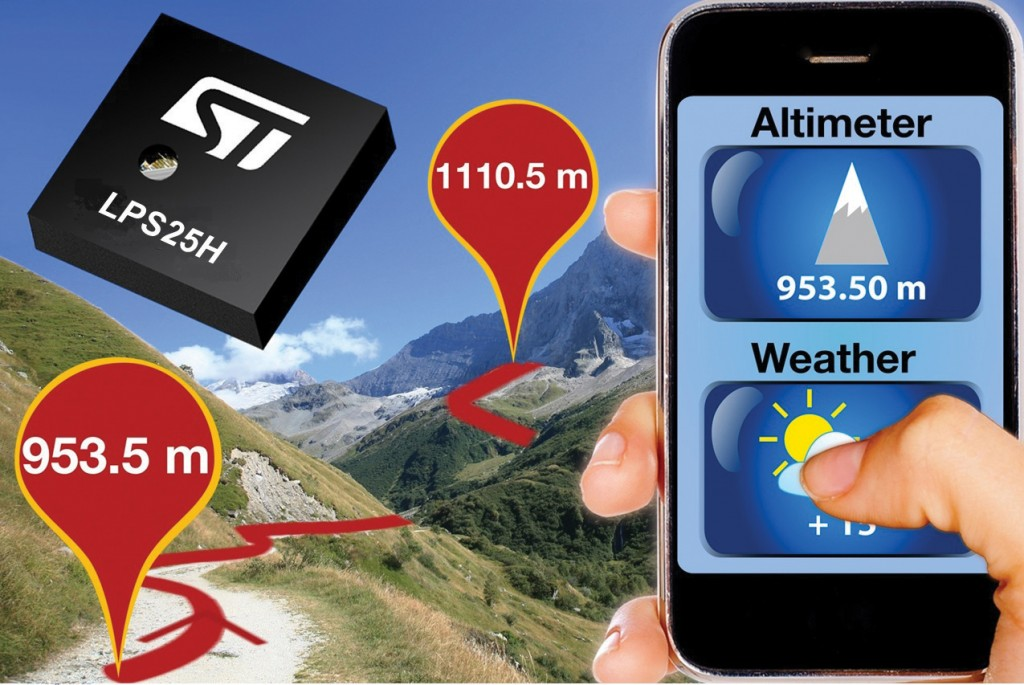
\includegraphics[scale=0.25]{LPS25H.jpg}
	\caption {STMicroelectronics LPS25H}
	\end{figure}

\item The LPS25H is an ultra compact absolute piezoresistive pressure sensor. It includes a
monolithic sensing element and an IC interface
able to take the information from the sensing
element and to provide a digital signal to the
external world.

\item The sensing element consists of a suspended
membrane realized inside a single mono-silicon
substrate. It is capable to detect the absolute
pressure and is manufactured with a dedicated
process developed by ST.

\item The membrane is very small compared to the
traditionally built silicon micromachined
membranes.Membrane breakage is prevented
by an intrinsic mechanical stopper.

\item The IC interface is manufactured using a standard
CMOS process that allows a high level of
integration to design a dedicated circuit which is
trimmed to better match the sensing element
characteristics.

\item The LPS25H is available in a cavity holed LGA
package (HCLGA). It is guaranteed to operate
over a temperature range extending from -30 degree Celsius
to +105 degree Celsius. The package is holed to allow
external pressure to reach the sensing element.

\item Applications
\begin{itemize}
\item Altimeter and barometer for portable devices
\item GPS applications
\item Weather Station Equipment
\item Sport Watches
\end{itemize}


\newpage
\section{Sensor 5 : Humidity and Temperature Sensor (HTS221)}
\begin{figure}[h]
    \centering
	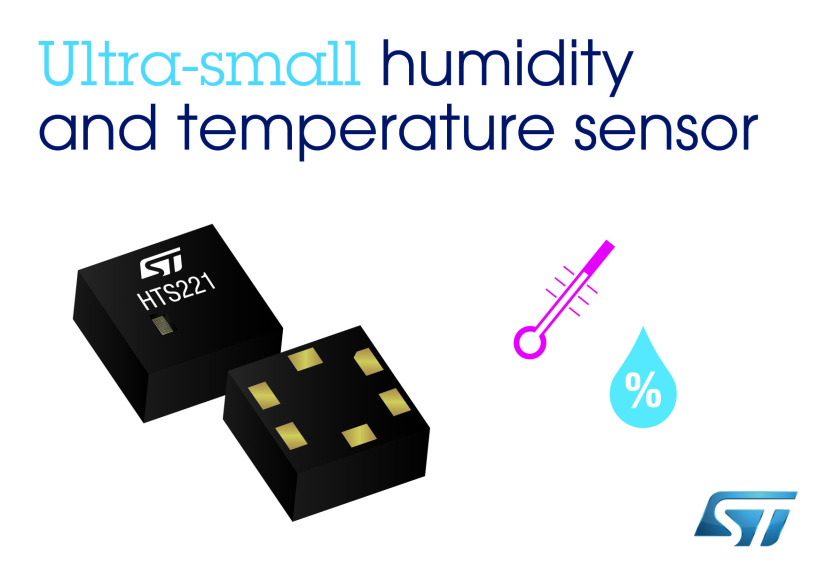
\includegraphics{HT.jpg}
	\caption {STMicroelectronics HTS221}
	\end{figure}
	
\item The HTS221 is an ultra compact sensor for
relative humidity and temperature. It includes a
sensing element and a mixed signal ASIC (Application-specific integrated circuit) to
provide the measurement information through
digital serial interfaces.
\item
The sensing element consists of a polymer
dielectric planar capacitor structure capable of
detecting relative humidity variations and is
manufactured using a dedicated ST process.
\item The HTS221 is available in a small top-holed cap
land grid array (HLGA) package guaranteed to
operate over a temperature range from -40 degree Celsius to
+120 degree Celsius.

\item Applications
\begin{itemize}
\item Air conditioning, heating and ventilation
\item Air humidifier
\item Refrigerators
\item Wearable devices 
\item Smart home automation
\item Industrial automation
\end{itemize}
 \end{itemize}





\newpage
	\section{References}
	 \begin{itemize}
	 \item https://community.cypress.com/community/wiced-smart
	 \item http://www.st.com/content/ccc/resource/technical/document/datasheet/4d/9a/9c/ad/25/07/\\42/34/DM00116291.pdf/files/DM00116291.pdf/jcr:content/translations/en.DM00116291.pdf
	 
	 \item http://www.st.com/content/st_com/en/products/mems-and-sensors/\\accelerometers/lis3dsh.html
	 
	
	     \end{itemize}
	    
\end{document}